\textbf{11.1.} 试由 $\omega$ 的单位: 秒 $^{-1}$ , $L$ 的单位: 亨利, $C$ 的单位: 法拉, 分别导出 $\omega L$ 、 $\frac{1}{\omega C} \sqrt{\frac{L}{C}}$ 等的单位.

\vfill

\textbf{11.2.} 一自感为 $L = 10\mathrm{H}$ , 一电容为 $C = 10\mu \mathrm{F}$ . (1) 试分别求频率为 $\nu = 50\mathrm{Hz}$ 和 $500\mathrm{Hz}$ 时它们的阻抗; (2) 在什么频率时它们的阻抗相等?

\vfill

\newpage

\textbf{11.3.} 自感为 $L = 31.8\mathrm{mH}$ 的线圈，其电阻可略去不计。当加上 $220\mathrm{V}, 50\mathrm{Hz}$ 的交流电压时，试求它的阻抗和通过它的电流。

\vfill

\textbf{11.4.} $C = 79.6\mu \mathrm{F}$ 的电容，接到 $220\mathrm{V},50\mathrm{Hz}$ 的交流电压上，试求它的阻抗和通过它的电流.

\vfill

\newpage

\textbf{11.5.} 在图 11.5 所示的十个电路中, R、L 和 C 都已知. 当用于角频率为 $\omega$ 的交流电路中时, 试分别求它们的阻抗 Z 和相角 $\varphi(\varphi = \varphi_{U} - \varphi_{I}, \quad \varphi_{U}$ 是该阻抗两端的电压的相位, $\varphi_{I}$ 是该阻抗中通过的电流的相位).

(9)RL 串联后与 C 并联

\vfill

\textbf{11.6.} 一个 R 和 L 串联电路, 接在电压为 100V 的交流电源上. (1) 一交流伏特计不论接在 R 两端还是接在 L 两端, 其读数都相等, 试问读数是多少? (2) 若改变 R 和 L 的大小, 使交流伏特计接在 L 两端时读数为 50V; 若将它接在 R 两端, 试问读数是多少?

\vfill

\newpage

\textbf{11.7.} 如图 11.7, 输电干线的电压为 U = 220V, 频率为 $\nu = 50.0Hz$ , 用户的照明电路与抗流线圈串联后接在两干线间. 抗流线圈的自感为 L = 50.0mH, 其电阻为 $r = 1.0\Omega$ . (1) 当用户用电 I = 2.00A 时, 试问电灯两端的电压是多少? (2) 用户电路(包括抗流线圈)能得到的最大功率是多少? (3) 当用户发生短路时, 抗流线圈中消耗的功率是多少?
\begin{center}
    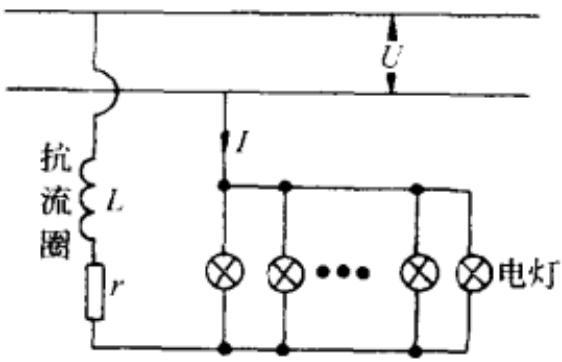
\includegraphics[width=0.5\linewidth]{figures/fig_11_7.jpg}
\end{center}

\vfill

\textbf{11.8.} — RC 串联电路, 接到 220V 50Hz 的交流电源上, 如图 11.8 所示. 现要求电流为 70mA, R 两端的电压为 8.0V, 试求 C 的值.

\vfill

\newpage

\textbf{11.9.} 在某个频率下,电容 C 和电阻 R 的阻抗之比为 $Z_{C}:Z_{R}=3:4$ . 现将它们串联后加上该频率的交流电压 U=100V. (1) 试分别求它们两端的电压 $U_{R}$ 和 $U_{C}$ ; (2) 试求电流 I 与电压 U 之间的相位差 $\varphi$ .

\vfill

\textbf{11.10.} 图 11.10 是一个 LC 滤波器, 已知频率 $\nu = 100Hz, C = 10\mu F$ . 现在要使输出的交流电压 $U_{2}$ 等于输入的交流电压 $U_{1}$ 的十分之一, 试求 L 的值.

\vfill

\newpage

\textbf{11.11.} 如图 11.11, 已知 C=300pF, 谐振频率 $\nu=1.0MHz$ . (1) 试求 L 的值; (2) 若 L 是一螺线管, 横截面的直径为 d=2.0cm, 相邻两匝间的距离为 0.50mm, 试求匝数 N.

\vfill

\textbf{11.12.} 一交流电路如图 11.12, 已知 $R = 20\Omega$ , 三个伏特计 $\mathbf{V}_1$ 的读数为 $U_1 = 44\mathrm{V}, \mathrm{V}_2$ 的读数为 $U_2 = 91\mathrm{V}, \mathrm{V}$ 的读数为 $U = 120\mathrm{V}$ . 试求元件 $Z$ 消耗的功率.

\vfill

\newpage

\textbf{11.13.} 一个 $110\mathrm{V}, 50\mathrm{Hz}$ 的交流电源, 向一负载 $Z$ 供电 $330\mathrm{W}$ , 负载的功率因数为 0.60, 电流的相位落后于电压. (1) 若在电路中串入一个电容 $C$ , 如图 11.13, 将功率因数提高到 1, 试求 $C$ 的值; (2) 这时电源供给的功率是多少?

\vfill

\textbf{11.14.} 有两个阻抗 $\widetilde{Z}_1 = R_1 + \mathrm{j}X_1$ 和 $\widetilde{Z}_2 = R_2 + \mathrm{j}X_2$ ，试证明：(1)当它们串联时，若通过它们的电流的有效值为 $I$ ，则它们消耗的功率便为 $P = I^2(R_1 + R_2)$ ；(2)当它们并联时，若通过它们的电流的有效值分别为 $I_1$ 和 $I_2$ ，则它们消耗的功率便为 $P' = I_1^2R_1 + I_2^2R_2$ .

\vfill

\newpage

\textbf{11.15.} 对于一个给定的交流电源来说,它的电动势和内阻抗都是一定的,设它的内阻抗为 $\widetilde{Z}_{i}=X+jY$ ,试证明:当负载的阻抗 $\widetilde{Z}$ 等于 $\widetilde{Z}_{i}$ 的共轭复数(即 $\widetilde{Z}=X-jY$ ,如图 11.15)时,电源输送到负载上的功率为最大.
\begin{center}
    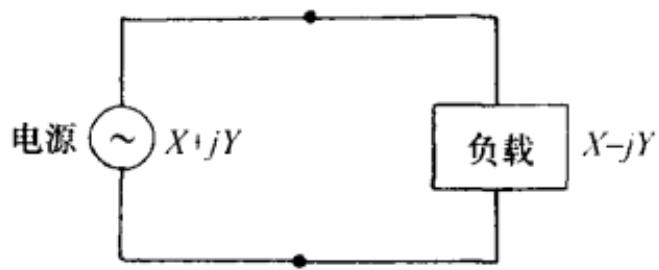
\includegraphics[width=0.5\linewidth]{figures/fig_11_15.jpg}
\end{center}

\vfill

\textbf{11.16.} 在用复数法解交流电路问题时,电压 $\widetilde{U}$ 、电流 $\widetilde{I}$ 和阻抗 $\widetilde{Z}$ 都用复数表示.对任何一个阻抗 $\widetilde{Z}$ 来说,它两端的电压 $\widetilde{U}$ 可由通过它的电流 $\widetilde{I}$ ,用复数形式的欧姆定律 $\widetilde{U} = \widetilde{I}\widetilde{Z}$ 求出.但它所消耗的功率 P 却不能由 $\widetilde{I}\widetilde{U}$ 求出.试证明:用复数表示时,瞬时功率为

$$
P (t) = \frac {1}{4} (\widetilde {I} \widetilde {U} + \widetilde {I} ^ {*} \widetilde {U} + \widetilde {I} \widetilde {U} ^ {*} + \widetilde {I} ^ {*} \widetilde {U} ^ {*})
$$

平均功率为

$$
P = \frac {1}{4} (\widetilde {I} ^ {*} \widetilde {U} + \widetilde {I} \widetilde {U} ^ {*})
$$

式中 $\widetilde{I}^{*}$ 和 $\widetilde{U}^{*}$ 分别是 $\widetilde{I}$ 和 $\widetilde{U}$ 的共轭复数，它们的模都是相应量的峰值.

\vfill

\newpage

\textbf{11.17.} — RLC 串联电路, 已知 $R = 400\Omega, L = 0.100\mathrm{H}, C = 0.500\mu \mathrm{F}$ . 试分别求频率为 $500\mathrm{Hz}$ 和 $1000\mathrm{Hz}$ 时的阻抗 $Z$ 和相角 $\varphi$ ; 试问加上电压后, 电流是落后还是超前?

\vfill

\textbf{11.18.} 一电路如图 11.18, 已知 $R_{1} = 6.0\Omega, R_{2} = R_{3} = 3.0\Omega$ ; 在 $\nu = 50\mathrm{Hz}$ 时, $X_{L} = 8.0\Omega, X_{C} = 3.0\Omega, U_{ab} = 130\mathrm{V}$ . 试求: (1) 电流 $I$ ; (2) $a$ 、 $c$ 两点间的电压 $U_{ac}$ ; (3) $c$ 、 $d$ 两点间的电压 $U_{cd}$ .

\vfill

\newpage

\textbf{11.19.} — RLC 串联电路如图 11.19, 已知 $R = 300\Omega$ , $L = 250\mathrm{mH}$ , $C = 8.00\mu \mathrm{F}$ , A 是交流安培计, $\mathrm{V}_{1}, \mathrm{V}_{2}, \mathrm{V}_{3}, \mathrm{V}_{4}$ 和 V 都是交流伏特计. 现将 $a, b$ 两端分别接到市电 (220V、50Hz) 电源的两极上. (1) 试问 A、 $\mathrm{V}_{1}, \mathrm{V}_{2}, \mathrm{V}_{3}, \mathrm{V}_{4}$ 和 V 的读数各是多少? (2) 试求 $a, b$ 间消耗的功率.

\vfill

\textbf{11.20.} 一 RLC 串联如图 11.19(见前面 11.19 题), 已知 $R = 300\Omega, L = 250\mathrm{mH}, C = 8.00\mu \mathrm{F}$ , A 是交流安培计, $\mathrm{V}_{1}, \mathrm{V}_{2}, \mathrm{V}_{3}, \mathrm{V}_{4}$ 和 V 都是交流伏特计. 现将 $a, b$ 两端加上 $220\mathrm{V}$ 、频率 $\nu$ 可变的交流电压. 试问 $\nu$ 为什么值时发生谐振? 这时 A、 $\mathrm{V}_{1}, \mathrm{V}_{2}, \mathrm{V}_{3}, \mathrm{V}_{4}$ 和 V 的读数各是多少?

\vfill

\newpage

\textbf{11.21.} 一 RLC 串联电路, 已知 $R = 5.00\Omega, L = 636\mathrm{mH}, C = 159\mu \mathrm{F}$ . 现在它两端加上 $U = 311\mathrm{V}, 50.0\mathrm{Hz}$ 的交流电压, 试求电路中的电流 $I$ 、电流 $I$ 与电压 $U$ 的相位差 $\varphi$ 以及各元件上的电压.

\vfill

\textbf{11.22.} 将已知的电阻 R、自感 L 和电容 C 串联后，接到一个恒压电源上，这电源的频率 $\nu$ 可以改变。(1)试求 L 两端电压最高时的频率 $\nu_{L}$ (用 R、L、C 等表示);(2)试求 C 两端电压最高时的频率 $\nu_{C}$ (用 R、L、C 等表示).

\vfill

\newpage

\textbf{11.23.} 一 RLC 串联电路, $R = 3.0\Omega$ , $C = 50\mu \mathrm{F}$ , $L$ 可以在 $10\mathrm{mH}$ 到 $80\mathrm{mH}$ 之间变化. 现在这电路两端加上有效值为 $U = 100\mathrm{V}$ 、角频率为 $\omega = 500\mathrm{rad/s}$ 的电压, 但 $C$ 两端电压的最大值不得超过 $1200\mathrm{V}$ . 试问这电路中最大容许电流的有效值是多少? $L$ 可以安全地增到多大?

\vfill

\textbf{11.24.} 一线圈的自感为 $L = 0.10\mathrm{H}$ , 电阻为 $R = 2.0\Omega$ , 与电容 $C$ 串联后接到 $\nu = 50\mathrm{Hz}$ 的交流电源上. (1) 试问 $C$ 为多大时线圈中的电流为最大? (2) 若这电容器的耐压为 $400\mathrm{V}$ , 试问电源的电压最大不能超过多少?

\vfill

\newpage

\textbf{11.25.} 一 RLC 串联电路, 已知 $R = 15\Omega$ , $C = 370pF$ , 谐振频率为 $\nu_{0} = 6.0 \times$

$10^{5}\mathrm{Hz}$ , 试求这电路的 $Q$ 值 $(Q = \frac{\omega_0L}{R})$ .

\vfill

\textbf{11.26.} 一个由元件 R、L、C 等联接而成的电路, 接在低压的交流电源上. 当 (1) 电路在谐振时, (2) 电源突然断开时, (3) 电源断开以后, 电路中都可能出现高压 (在用电时应注意这点). 试说明出现高压的原因.

\vfill

\newpage

\textbf{11.27.} 一 RLC 串联电路的谐振频率为 $\nu_{0}$ ，试证明，当这电路中的频率与 $\nu_{0}$ 相差为 $\Delta\nu$ ，而 $\Delta\nu\ll\nu_{0}$ 时，它的阻抗近似为 $Z=R\sqrt{1+\left(2Q\frac{\Delta\nu}{\nu_{0}}\right)^{2}}$ ，式中 $Q=\frac{\omega_{0}L}{R}=\frac{2\pi\nu_{0}L}{R}$ 是这电路的 Q 值（品质因数）.

\vfill

\textbf{11.28.} RLC 串联电路的谐振频率为 $\nu_0 = \frac{1}{2\pi}\frac{1}{\sqrt{LC}}$ ，试推导这个公式。有一发射天线发出的电磁波的频率为 $1.25\mathrm{MHz}$ ，试求它的振荡电路的 $LC$ 值。

\vfill

\newpage

\textbf{11.29.} 超外差式收音机里的中周谐振频率是 465kHz, 在它的调谐回路里, 电容常用 200pF. 试问这时中周线圈的自感是多少?

\vfill

\textbf{11.30.} 一 RLC 串联电路, $R = 5.0\Omega, Z_{L} = 20\Omega, Z_{C} = 20\Omega$ , 加上 $100\mathrm{V}$ 的交流电压, 试求发生谐振时电路中的电流和 $R, L, C$ 上的电压.

\vfill

\newpage

\textbf{11.31.} $R_{1}L_{1}C_{1}$ 串联电路的谐振频率与 $R_{2}L_{2}C_{2}$ 串联电路的谐振频率相等，如果将这两个电路串联起来，而 $L_{1}$ 与 $L_{2}$ 之间的互感可略去不计，试问整个电路的谐振角频率是多少？

\vfill

\textbf{11.32.} $R = 10.0\Omega$ 与 $L = 31.8\mathrm{mH}$ 并联后，加上 $u(t) = 156\sin \omega t\mathrm{V},\nu = \omega /2\pi = 100\mathrm{Hz}$ 的电压，如图11.32(1)所示.试求通过 $R$ 的电流 $i_R(t)$ ，通过 $L$ 的电流 $i_L(t)$ 和总电流 $i(t)$

\vfill

\newpage

\textbf{11.33.} 一抗流圈的自感为 $L = 50\mathrm{mH}$ 、电阻为 $r = 20\Omega$ ，与 $R = 60\Omega$ 的变阻器并联后，接到 $\nu = 50\mathrm{Hz}$ 的交流电源上，如图11.33(1)所示.测得通过 $L$ 的电流为 $I_{L} = 4.0\mathrm{A}$ ，试求通过 $R$ 的电流 $I_{R}$ 和总电流 $I$

\vfill

\textbf{11.34.} 一电路如图 11.34(1)，已知 $R = 50\Omega, I_{R} = 2.5A, I_{Z} = 2.8A, I = 4.5A$ ，试求元件 Z 所消耗的功率.

\vfill

\newpage

\textbf{11.35.} 一电器的工作频率为 $50\mathrm{Hz}$ , 功率因数为 0.70, 有功电阻为 $100\Omega$ . 试问并联一个多大的电容 $C$ , 可以使整个电路的功率因数提高到 1?

\vfill

\textbf{11.36.} 一 RC 并联电路如图 11.36 所示. 已知 R、C 和电压 $u(t) = U_{0} \cos \omega t$ ，试求电流 $i(t)$ .

\vfill

\newpage

\textbf{11.37.} 一交流电路如图 11.37(1)，已知 $R = 5.0k\Omega, C = 0.010\mu F$ . 试分别求 $(1)\nu = 465Hz$ 和 $(2)\nu = 10kHz$ 时的比值 $I_{R}/I$ .

\vfill

\textbf{11.38.} 如图 11.38(1), RC 并联电路的阻抗, 在 $\omega CR \gg 1$ 时, 近似等于 $C' = C$ 与 $R' = \frac{1}{\omega^{2} C^{2} R}$ 串联电路 [如图 11.38(2)] 的阻抗. 试证明上述结论.

(1)

(2)
\begin{center}
    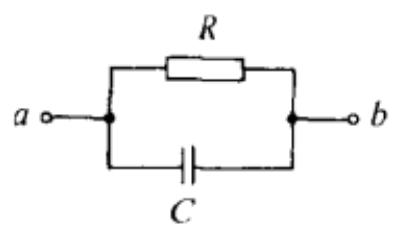
\includegraphics[width=0.5\linewidth]{figures/fig_11_38_1.jpg}
\end{center}
\begin{center}
    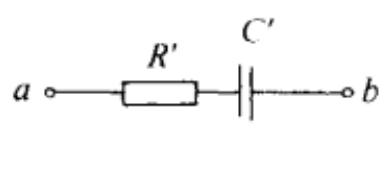
\includegraphics[width=0.5\linewidth]{figures/fig_11_38_2.jpg}
\end{center}

\vfill

\newpage

\textbf{11.39.} 交电流通过电阻 R. 与 R 并联一电容 C 后, 设电流的大小不变(即通过并联电路的总电流等于未并联 C 时通过 R 的电流), (1) 试问 R 上的电压降低了多少? (2) 若 $R = 30k\Omega, C = 0.33\mu F$ , 试问在什么频率时, R 上的电压下降 5%?

\vfill

\textbf{11.40.} 一 LC 并联电路, 在某个频率时, L 和 C 的阻抗之比为 $Z_{L}:Z_{C}=2:1$ , 通过这并联电路的总电流为 I=1.0 毫安. 试分别求通过 L 的电流 $I_{L}$ 和通过 C 的

电流 $I_{C}$ .

\vfill

\newpage

\textbf{11.41.} 中波收音机的输入调谐回路由一可变电容 C 与环式线圈 L 串联而成，C 的变化范围为 30pF 到 300pF，L 则是将外表绝缘的细导线绕在铁氧体环上构成，已知铁氧体的 $\mu_{r}=200$ ，磁路长为 3.0cm，横截面积为 0.10 平方厘米，导线横截面的直径为 0.50mm，电阻率为 $1.7\times10^{-8}\Omega\cdot m$ 。(1) 如果想收听 500kHz 到 1500kHz 波段的电台，试问 L 应该有多少匝？(2) 当收听 1151kHz 的节目时，1214kHz 的串音是否严重？

\vfill

\textbf{11.42.} 试证明: 在谐振时, LC 串联的阻抗为 $\infty$ , LC 并联的阻抗为零.

\vfill

\newpage

\textbf{11.43.} 一 RLC 并联电路如图 11.43(1)，已知 $R = 300\Omega, L = 250mH, C = 8.00\mu F; A_{1}, A_{2}, A_{3}, A_{4}$ 和 A 都是交流安培计，它们本身的阻抗都很小，可略去不计。现在 a、b 两端加上 220V、50Hz 的交流电压，试求：(1) 五个安培计的读数；(2) $A_{4}$ 中的 $I_{RL}$ 与 $U_{ab}$ 的相位差；(3) a、b 间所消耗的功率。

图11.43(1)
\begin{center}
    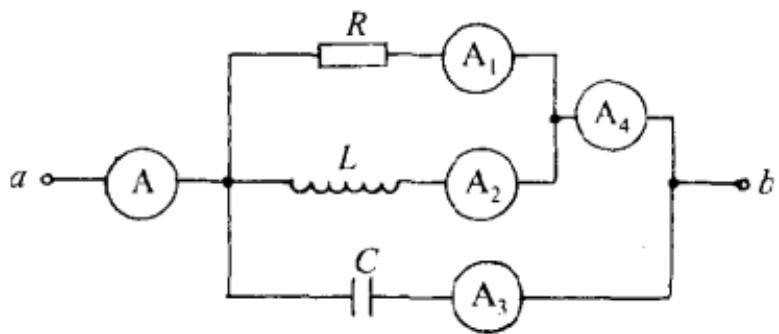
\includegraphics[width=0.5\linewidth]{figures/fig_11_43.jpg}
\end{center}

\vfill

\textbf{11.44.} — RLC 并联电路如图 11.44(1)，其中 R、L、C、U 和 U 的角频率 $\omega$ 都已知，试求：(1) 电流 $I_{1}$ 、 $I_{2}$ 、 $I_{3}$ 和 I；(2) I 与 $I_{2}$ 之间以及 I 与 $I_{3}$ 之间的相位差.

\vfill

\newpage

\textbf{11.45.} — RLC 并联电路如图 11.45, 试证明: 在谐振频率 $\nu_{0}$ 附近, 这电路的导纳(阻抗的倒数)近似等于 $\widetilde{Y} = \frac{1}{R} + 2jC\delta\omega$ , 式中 $\delta\omega = \omega - \omega_{0} = 2\pi(\nu - \nu_{0})$ .

\vfill

\textbf{11.46.} 一电路如图 11.46, 其中 R、r、L 和 C 均已知, 试求电路的谐振频率.

\vfill

\newpage

\textbf{11.47.} 在频率为 $\nu = 50\mathrm{Hz}$ 的交流电路中，电阻 $R$ 与一个线圈串联，这线圈的自感为 $L = 0.10\mathrm{H}$ ，其电阻可略去不计。通过这电路的电流与加在它两端电压的相位差为 $\varphi = 30^{\circ}$ 。（1）试求 $R$ 的值；(2)若在这电路两端并联一个电容 $C$ ，以消除上述相位差，试求 $C$ 的值；(3)若在这电路中串入一个电容 $C'$ ，以消除上述相位差，试求 $C'$ 的值。

\vfill

\textbf{11.48.} 在 $RL$ 串联电路两端加上 $U = 220\mathrm{V}, \nu = 50\mathrm{Hz}$ 的市电, 已知 $R = 6.0\Omega$ , 感抗 $X_{L} = 8.0\Omega$ . 现在想要将功率因数提高到 0.95, 试问: (1) 应在这电路两端并联多大的电容? (2) 应在这电路中串入多大的电容?

\vfill

\newpage

\textbf{11.49.} 一个 $RL$ 串联后再与 $C$ 并联的电路如图11.49, 其中电阻 $R$ 、电感 $L$ 和电容 $C$ 以及电源的角频率 $\omega$ 都已知. 试求下列两点间电流与电压的相位差: (1) $a, b$ ; (2) $b, c$ ; (3) $a, c$ ; (4) $d, e$ ; (5) $f, g$ .

$$
\text {   【解   】   } \quad (1) \varphi_ {a b} = \varphi_ {U} - \varphi_ {I} = \arctan \left(\frac {X}{R}\right) = \arctan 0 = 0
$$

$$
(2) \varphi_ {b c} = \varphi_ {U} - \varphi_ {I} = \arctan \left(\frac {X}{r}\right) = \arctan \left(\frac {\omega L}{0}\right) = \frac {\pi}{2}
$$

$$
\varphi_ {a c} = \varphi_ {U} - \varphi_ {I} = \arctan \left(\frac {X}{R}\right) = \arctan \left(\frac {\omega L}{R}\right) \tag {3}
$$

$$
\varphi_ {d e} = \varphi_ {U} - \varphi_ {I} = \arctan \left(\frac {X}{r}\right) = \arctan \left(\frac {\frac {1}{\omega C}}{0}\right) = - \frac {\pi}{2} \tag {4}
$$

(5)
\begin{center}
    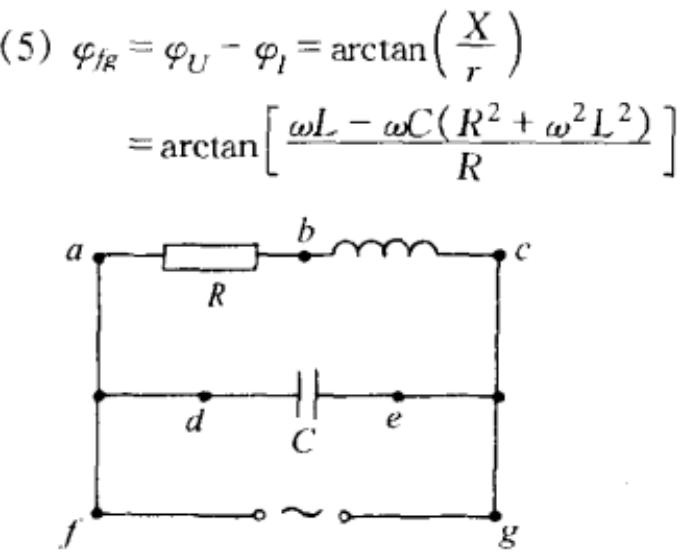
\includegraphics[width=0.5\linewidth]{figures/fig_11_49_1.jpg}
\end{center}
\begin{center}
    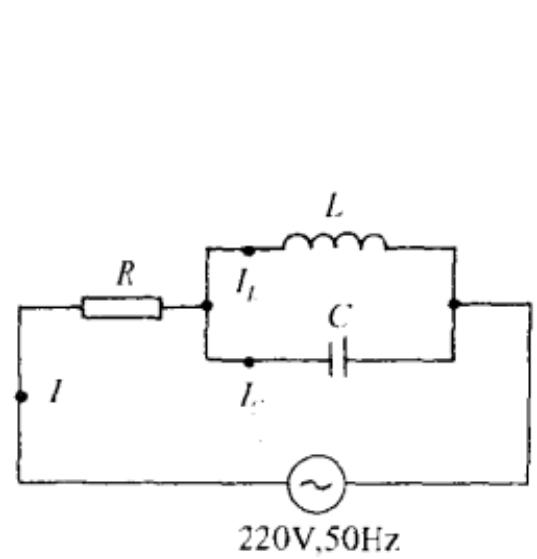
\includegraphics[width=0.5\linewidth]{figures/fig_11_49_2.jpg}
\end{center}

\vfill

\textbf{11.50.} 一交流电路如图 11.50, 已知 $R = 8.0\Omega, L = 9.55\mathrm{mH}, C = 530\mu \mathrm{F}$ , 交流电源的电压为 $220\mathrm{V}$ , 频率为 $50\mathrm{Hz}$ . (1) 试分别求 $L$ 和 $C$ 的阻抗 $Z_{L}$ 和 $Z_{C}, LC$ 并联的阻抗 $Z_{LC}$ , 以及整个 $RLC$ 电路的阻抗 $Z$ ; (2) 试求电流 $I_{L}, I_{C}$ 和 $I$ ; (3) 试求 $R$ 两端的电压 $U_{R}$ 和 $LC$ 两端的电压 $U_{LC}$ .

\vfill

\newpage

\textbf{11.51.} 一 $\pi$ 形滤波电路如图11.51, 已知 $C_1 = C_2 = 10\mu \mathrm{F}, \nu = 100\mathrm{Hz}$ . 要求输出电压 $U_2$ 为输入电压 $U_1$ 的 $\frac{1}{10}$ , 试求 $L$ 的值.

\vfill

\textbf{11.52.} 一交流电路如图 11.52, 设电阻 R、电感 L、电容 C 和电压 U 的角频率 $\omega$ 均为已知, 试求: (1) $I_{1}$ 与 $I_{2}$ 的相位差; (2) $U_{C}$ 与 U 的相位差.

\vfill

\newpage

\textbf{11.53.} 一交流电路如图 11.53, 其中 R、r、L、C、U 和 U 的角频率 $\omega$ 都已知, 试求下列各量间的相位差: (1) $U_{C}$ 与 $I_{R}$ ; (2) $I_{C}$ 与 $I_{R}$ ; (3) $U_{R}$ 与 U.

\vfill

\textbf{11.54.} 图 11.54 是为消除分布电容而设计的一种脉冲分压器, 要使输出电压 $U_{2}$ 与输入电压 $U_{1}$ 之比等于电阻之比 [即 $U_{2}/U_{1}=R_{2}/(R_{1}+R_{2})$ ] 而与频率无关, 试问 $R_{1}, R_{2}, C_{1}, C_{2}$ 等应满足什么关系?

\vfill

\newpage

\textbf{11.55.} RC 振荡器的电路如图 11.55 所示, 当总电压 $u(t)$ 与分电压 $u_{2}(t)$ 的相位相同时, 电路中的频率称为振荡频率, 以 $\nu_{0}$ 表示. 试证明: (1) $\nu_{0} = \frac{1}{2\pi RC}$ ;

(2) 当 $\nu = \nu_0$ 时, $u(t)$ 与 $u_2(t)$ 的峰值的关系为 $U_0 = 3U_{20}$ .

\vfill

\textbf{11.56.} 交流电路中的一部分如图 11.56 所示，当 $R_{1}$ 或 $R_{2}$ 发生变化时，试问 $I_{1}$ 与 $I_{2}$ 之间的相位差是否发生变化？

\vfill

\newpage

\textbf{11.57.} 在一环形铁心上绕有 $N$ 匝外表绝缘的导线, 导线两端接到电动势为 $\varepsilon$ 的交流电源上. 一电阻为 $R$ 、自感可略去不计的均匀细圆环套在这环形铁芯上, 细圆环上 $a, b$ 两点间的环长 (劣弧) 为细圆环长度的 $\frac{1}{n}$ . 将电阻为 $r$ 的交流电流计 $G$ 接在 $a, b$ 两点, 有两种接法, 分别与图 11.57(1) 和 (2) 所示. 试分别求这两种接法时通过 $G$ 的电流.

(1)

(2)
\begin{center}
    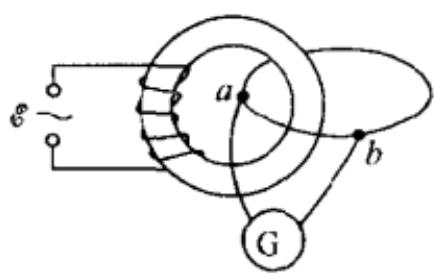
\includegraphics[width=0.5\linewidth]{figures/fig_11_57_1.jpg}
\end{center}
\begin{center}
    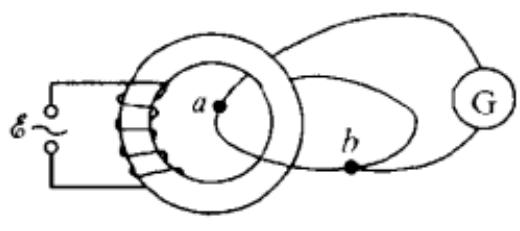
\includegraphics[width=0.5\linewidth]{figures/fig_11_57_2.jpg}
\end{center}

\vfill

\textbf{11.58.} 一交流电桥的电路如图 11.58(1)，其中 $\widetilde{Z}_{1}$ 、 $\widetilde{Z}_{2}$ 、 $\widetilde{Z}_{3}$ 和 $\widetilde{Z}_{4}$ 分别为四个臂的复阻抗；当交流检电流计 G 中无电流通过时，交流电桥便达到平衡。试证明：交流电桥的平衡条件为 $\widetilde{Z}_{2}\widetilde{Z}_{3}=\widetilde{Z}_{4}\widetilde{Z}_{1}$ 。

\vfill

\newpage

\textbf{11.59.} 图 11.59 中的(1)和(2)分别是两种交流电桥,试分别求它们各自的平衡条件.

(1)

(2)
\begin{center}
    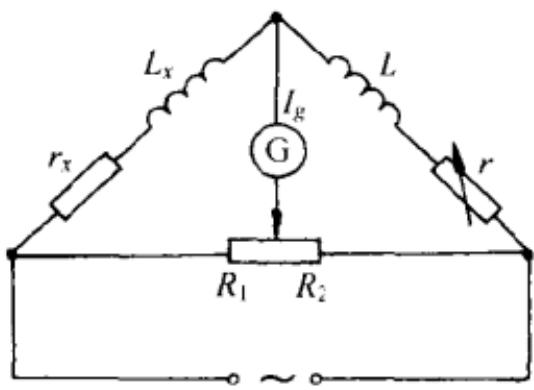
\includegraphics[width=0.5\linewidth]{figures/fig_11_59_1.jpg}
\end{center}
\begin{center}
    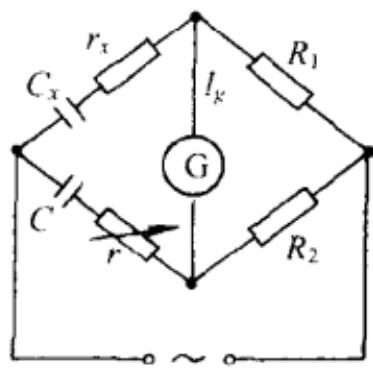
\includegraphics[width=0.5\linewidth]{figures/fig_11_59_2.jpg}
\end{center}

\vfill

\textbf{11.60.} 麦克斯韦电桥是用来测量自感和电容的装置, 它的电路如图 11.60 所示. 为了使电桥达到平衡, 其中 $R_{4}$ 和 C 都是可变的. 试证明: 它的平衡条件为: $R_{2}R_{3}=R_{4}R_{1}$ 和 $L=R_{2}R_{3}C$ .

\vfill

\newpage

\textbf{11.61.} 奥温(Owen)电桥的线路如图 11.61 所示, 其中 $R_{1}$ 和 $R_{3}$ 都是可变的, 用于调节平衡. 试求这电桥的平衡条件.

\vfill

\textbf{11.62.} 图 11.62 是测量交流电频率的电桥, 其中电阻 $R_{3}$ 和 $R_{4}$ 、电感 L 和电容 C 都是可变的, 用以调节电桥的平衡. 试求这电桥的平衡条件, 从而导出所测交流电的频率.

\vfill

\newpage

\textbf{11.63.} 一变压器的原线圈为 660 匝, 接在 220V 的交流电源上, 测得三个副线圈的电压分别为 (1)5V, (2)6.3V 和 (3)350V. 试分别求它们的匝数. 设这三个副线圈中的电流分别为 (1)3A, (2)3A 和 (3)280mA, 试问通过原线圈的电流是多少?

\vfill

\textbf{11.64.} 要将一个输入 220V、输出 6.3V 的变压器，改绕成输入 220V、输出 30V 的变压器；现拆出它的次级线圈，数出圈数为 38 匝，试问应改绕成多少匝？

\vfill

\newpage

\textbf{11.65.} 两用变压器是一种既可用 220V 电源,也可用 110V 电源的变压器,其结构如图 11.65 所示,原线圈是由两组完全相同的线圈 1、2 和 3、4 构成的.在用 220V 电源时,将 2 和 3 接在一起,再将 1 和 4 分别接到 220V 电源的两极上;在用 110V 电源时,将 1 和 3 接在一起,2 和 4 接在一起,然后分别接到 110V 电源的两极上.在这两种情况下,副线圈的电压都相同,即都是 280V 和 6.3V.试说明它的道理.

\vfill

\textbf{11.66.} 自耦变压器是绕在铁心上的一个线圈, 按一定的匝数分别接出一些线头而成, 如图 11.66 所示. 已知 $a, b$ 间为 100 匝, $b, c$ 间为 200 匝, $c, d$ 间为 300 匝, $d, e$ 间为 400 匝. 当 $a, e$ 间加上 $U_{ae} = 120\mathrm{V}$ 的交流电压时, 试求 $U_{ab}, U_{ac}, U_{bc}$ 和 $U_{de}$ .

\vfill

\newpage

\textbf{11.67.} 一升压变压器将 100V 的交流电压升高到 3300V. 现将一条导线套住变压器的铁心接在交流伏特计 V 上, 如图 11.67 所示, 这伏特计的读数为 0.50V. 试问这变压器两绕组的匝数各是多少?

\vfill

\textbf{11.68.} 一交流讯号电源的电动势为 $\mathcal{E}=6.0V$ ，内阻为 $r=100\Omega$ ;一扬声器的电阻为 $R=8.0\Omega$ . (1) 将讯号电源直接接到扬声器上, 如图 11.68(1) 所示, 试求讯号电源的输出功率; (2) 讯号电源通过一耦合变压器(原线圈匝数为 $N_{1}=350$ , 副线圈匝数为 $N_{2}=100$ ) 接到扬声器上, 如图 11.68(2) 所示, 试求这时讯号电源的输出功率.
\begin{center}
    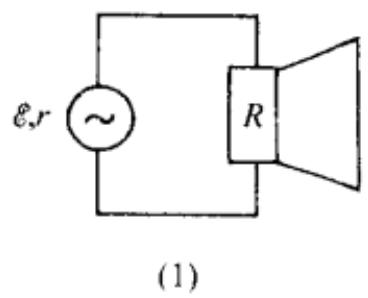
\includegraphics[width=0.5\linewidth]{figures/fig_11_68_1.jpg}
\end{center}
\begin{center}
    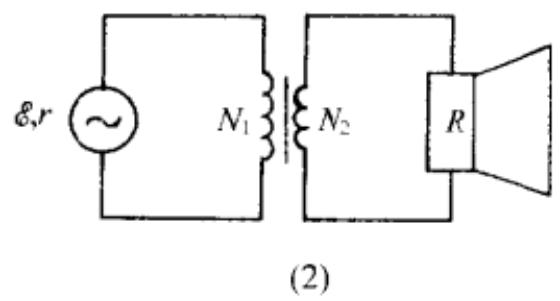
\includegraphics[width=0.5\linewidth]{figures/fig_11_68_2.jpg}
\end{center}

\vfill

\newpage

\textbf{11.69.} 一同轴电缆由半径为 $a$ 的长直导线和与它同轴的导体薄圆筒构成，圆筒的半径为 $b$ . 在导线与圆筒间充满介电常数为 $\varepsilon_{\mathrm{r}}$ 、相对磁导率为 $\mu_{\mathrm{r}}$ 的均匀介质. 电缆在使用时，电流均匀分在导线和圆筒的横截面上. 电缆的特性阻抗定义为 $Z_0 = \sqrt{L_1 / C_1}$ ，式中 $L_{1}$ 为单位长度的自感， $C_{1}$ 为单位长度的电容. 略去导线内的磁通量. (1) 试求这电缆的特性阻抗 $Z_0$ ; (2) 很多实用电缆都采用 $Z_0 = 50\Omega$ (有时称为 $50\Omega$ 电缆), 设其中介质为 $\varepsilon_{\mathrm{r}} = 2.3, \mu_{\mathrm{r}} = 1$ 的聚乙烯, 试计算 $b / a$ 的值.

\vfill

\textbf{11.70.} 平行导体片传输线的一段如图 11.70 所示, 两导体薄片的宽度都是 $a$ , 相距为 $b$ , 中间充满介电常数为 $\varepsilon_{r}$ 、相对磁导率为 $\mu_{r}$ 的均匀介质. 使用时, 电流沿长度方向流动, 从一片流去, 另一片流回. 设电流在两片上都是均匀分布, 并略去边缘效应. 这传输线的特性阻抗定义为 $Z_{0} = \sqrt{L_{1} / C_{1}}$ , 式中 $L_{1}$ 是单位长度的自感, $C_{1}$ 是单位长度的电容. 试证明: $Z_{0} = \sqrt{\frac{\mu_{r} \mu_{0}}{\varepsilon_{r} \varepsilon_{0}}} \frac{b}{a}$ .
\begin{center}
    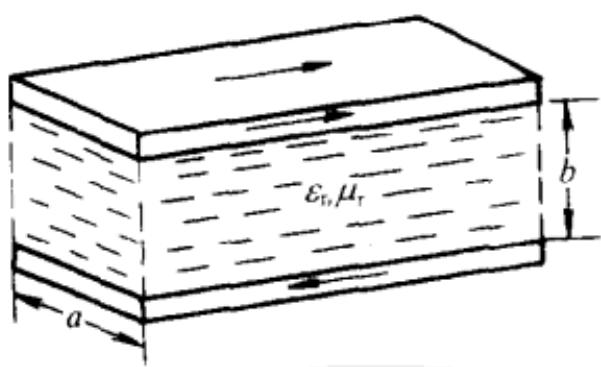
\includegraphics[width=0.5\linewidth]{figures/fig_11_70.jpg}
\end{center}

\vfill

\newpage

\textbf{11.71.} 一星形联接的三相对称负载(电动机), 每相的电阻为 $R = 6.0\Omega$ , 电抗为 $X = 8.0\Omega$ ; 电源的线电压为 $380\mathrm{V}$ , 如图 11.71 所示.(1)试求线电流和负载所消耗的功率;(2)如果改接成三角形, 试求线电流和负载所消耗的功率.

\vfill

\textbf{11.72.} 三相交流电的线电压为 $380\mathrm{V}$ , 负载是不对称的纯电阻, $R_{A} = R_{B} = 22\Omega, R_{C} = 27.5\Omega$ , 如图 11.72(1)所示. (1)试求中线电流和负载上各相的相电压; (2)若中线断开, 负载上各相的电压将变为多少?

\vfill

\newpage
